This section introduces the concept of disguised data by illustrating how
developers and users would interact with an application that supports 
data disguising and data revealing.
%

\begin{figure}[h!]
  \centering
    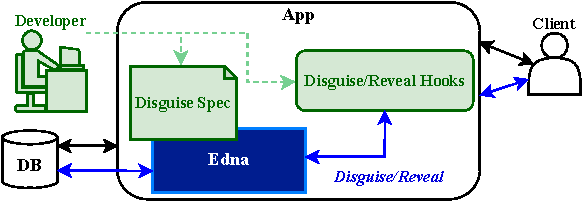
\includegraphics{figs/edna_overview}
    \caption{Developers write \xx specifications and add hooks to invoke \sys
        from the application (green); in normal operation, clients use these
        hooks in the application to \xx and reveal their data in the database
        (blue).
    }
  \label{f:edna-overview}
\end{figure}
%
\sys helps developers realize new options for users to control their data
via \emph{\xxing transformations}; and add support for users to invoke
\emph{revealing transformations}
%
The developer integrates an application with \sys by writing \xx specifications
and adding hooks to \xx or reveal data using \sys's API
(Figure~\ref{f:edna-overview}).
%
This proceeds as follows:
%

%
(1) An application registers users with a public--private keypair
that either the application or the user's client generates; \sys stores the
public key in its database, while the user retains the private key for use in
future reveal operations.
%

%
(2) When the application wants to \xx some data, it invokes \sys with the
corresponding developer-provided \xx specification and any necessary
parameters (such as a user ID).
%
\Xx specifications can remove data, modify data (replacing some or all of its
contents with placeholder values), or decorrelate data, replacing
links to users with links to pseudoprincipals (fake users).
%
% Decorrelation preserves the structure of the application database, and avoids
% integrity issues like dangling foreign keys, while obscuring the data's
% relationship to natural principals (true users).
%
\sys takes the data it removed or replaced and the connections between
the user and any pseudoprincipals it created, encrypts that data with the user's
public key, and stores the resulting ciphertext---the \emph{\xxed
data}---such that it cannot be linked back to the user without the user's
private key.
%
%The application's database now no longer contains the \xxed data.
%

%
\todo{check} 
(3) If the developer decides to update application contents (\eg by performin a
global moderation or a schema migration), then the developer writes
an \emph{application update executable} that encapsulate these changes applied to
a single user's data, and invokes \sys's API to record this update. \sys then
uses these executables to reveal disguised data without overwriting the
associated application changes.
%

%
(4) When a user wishes to reveal their \xxed data, they pass credentials
to the application, which calls into \sys to reveal the data.
%
Credentials are application-specific: users may either provide their private
key or other credentials sufficient for \sys to re-derive the private key.
%
\sys reads the \xxed data and decrypts it, undoing the changes to the
application database that \xxing introduced.
%

%
\sys provides the developer with sensible default \xxing and revealing
semantics (\eg revealing makes sure not to overwrite changes made since
\xxing).


%%%%%%%%%%%%%%%%%%%%%%%%%%%%%%%%%%%%%%%%%%%%%%%%%%%%%%%%%%%%%%
\section{Example: Lobsters Topic Anonymization}
\label{s:design:lobsters}

\begin{figure}[t]
\centering
\begin{lstlisting}[style=rust,escapeinside={(*}{*)}]
// Decorrelate comments on stories w/tag {{TAG}}
"comments": [{
  "type": "Decorrelate",
  "predicate": "tags.tag = {{TAG}}",
  "from": "comments JOIN stories ON comments.story_id = stories.id
           JOIN taggings ON stories.id = taggings.story_id
           JOIN tags ON...",
  "group_by": "stories.id",
  "principal_fk": "comments.user_id" } ],
// Remove votes on stories w/tag {{TAG}}
"votes": [{
  "type": "Remove",
  "predicate": "tags.tag = {{TAG}}",
  "from": "votes JOIN stories...",
  "principal_fk": "votes.user_id",
}, ... ]
\end{lstlisting}
    \caption{Lobsters topic-based anonymization \xx specification (JSON
    pseudocode), which decorrelates comments and removes votes on stories with
    the specific topic tag.}
\label{f:spec}
\end{figure}

\begin{figure}[h]
  \centering
  \begin{subfigure}[h]{0.5\columnwidth}
  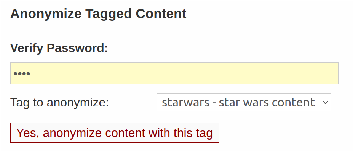
\includegraphics[width=\columnwidth]{figs/lobsters_catanon}
  \end{subfigure}
  \begin{subfigure}[h]{\columnwidth}
  \begin{lstlisting}[language=Ruby,escapeinside={(*}{*)}]
  def tag_anon
    # instantiate the disguise spec with the provided tag to anonymize
    disg_spec = edna.instantiate_spec("tag_anon.json",params[:tag])
    # apply the disguising transformation
    disg_id = edna.apply_disguise(@user.id,params[:passwd],disg_spec)
    # email the disguise ID to the user to allow revealing
    SendDisguiseEmail(@user, disg_id)
  end
  \end{lstlisting}
  \end{subfigure}
  \vspace*{-1em}
  \caption{The Lobsters developer adds a hook in the UI and code to perform
      topic-based anonymization.}
  \label{f:lobsters_hook}
  \end{figure}

We next describe how \sys's API and \xx specifications work via a \xxing
transformation for Lobsters~\cite{lobsters}.  Lobsters~\cite{lobsters} is a
link-sharing and discussion platform with 15.4k
users.
%
Its database schema consists of stories, tags on stories, comments, votes,
private messages, user accounts, and other user-associated metadata.
%
Users create accounts, submit URLs as stories, and interact with other users
and their posted stories via comment threads and votes.
%

Consider \textbf{topic-based anonymization}, which allows users to
hide their interest in a topic (a ``tag'' in Lobsters) by decorrelating
their comments and removing their votes on stories with that tag.
%
For instance, a Lobsters user Bea who posts about their interests---Rust,
static analysis, and Star Wars---might want to hide associations with
Star Wars before sharing their profile with potential employers.
%
This is currently not possible in Lobsters.

%
The Lobsters developer can realize topic-based anonymization as a \xxing
transformation.
% that anonymizes Bea's contributions in the database, while allowing
% Bea to later edit and reclaim them if desired.
%
First, the developer writes a \xx specification that instructs \sys to
decorrelate comments and remove votes on ``Star Wars'' stories
(Figure~\ref{f:spec}), and provides it to \sys.
%
They also add frontend code and UI elements that allow authenticated users to
trigger the \xxing transformation (Figure~\ref{f:lobsters_hook}).
%
When Bea wants to anonymize their contributions on content tagged ``Star Wars,''
Lobsters invokes \sys with the provided specification.

\todo{xxx}
If the developer performs a global application change that \eg normalizes the
URLs of stories, the developer performs a bulk update in the Lobsters
applications. The developer also writes an update executable encoding how to
update individual user's stories' URLs as well. Then the developer invokes
\sys's \texttt{record\_update} API call with the update executable.
%

%
When Bea wants to deanonymize their ``Star Wars'' contributions, Lobsters
invokes \sys with Bea's reveal credentials and the disguise ID, and \sys reveals
Bea's associations with ``Star Wars'' posts, applying application updates and
schema migrations while doing so.
%

%%%%%%%%%%%%%%%%%%%%%%%%%%%%%%%%%%%%%%%%%%%%%%%%%%%%%%%%%%%%%%%%
%\section{Design}

\section{Disguise Specifications}
\label{s:spec}

\sys's developer interface is designed so that developers need to reason only
about the high-level semantics of disguising expressed in the disguise
specification. \sys takes care of applying disguise transformations, composing
it with other disguising and revealing transformations, and creating and storing
disguised data.


\begin{figure}[t]
\centering
\begin{lstlisting}[style=rust,escapeinside={(*}{*)}]
// Decorrelate comments on stories w/tag {{TAG}}
"comments": [{
  "type": "Decorrelate",
  "predicate": "tags.tag = {{TAG}}",
  "from": "comments JOIN stories
           ON comments.story_id = stories.id
           JOIN taggings
           ON stories.id = taggings.story_id
           JOIN tags ON...",
  "group_by": "stories.id",
  "principal_fk": "comments.user_id" } ],
// Remove votes on stories w/tag {{TAG}}
"votes": [{
  "type": "Remove",
  "predicate": "tags.tag = {{TAG}}",
  "from": "votes JOIN stories...",
  "principal_fk": "votes.user_id",
}, ... ]
\end{lstlisting}
    \caption{Lobsters topic-based anonymization \xx specification (JSON
    pseudocode), which decorrelates comments and removes votes on stories with
    the specific topic tag.}
\label{f:spec}
\end{figure}

%For every \xxing transformation, the developer writes a \xx specification
%(Figure~\ref{f:spec})
\Xx specifications tell \sys what application data objects to \xx and how to \xx them.
%
A \xx specification identifies objects by database table name, principal, and
predicate, where a predicate is a SQL \fn{WHERE} clause.
%
\sys by default \xxs all objects related to the given principal, as defined by
a foreign-key relationship provided in the \xx specification (using
\texttt{principal\_fk}), but predicates can narrow the transformation's scope
(\eg to stories with specific tags).
%
For each selected group of objects, developers choose to
\emph{remove}, \emph{modify}, or \emph{decorrelate} them.
%, replacing some or all of their contents with placeholder values;
%or \three{} \emph{decorrelate} them.
%where decorrelation removes associations between principals and objects and
%re-associates the objects with pseudoprincipals. \hmng{this is a pretty verabtim
%repetition from section 3, remove or condense I'd say?}
%
The example specification in Figure~\ref{f:spec} decorrelates all comments and removes all
votes on stories with a particular tag, specified by the \texttt{TAG} parameter provided
at invocation time.
%
%or a custom set of objects specified by the \xxing transformation.
%\lyt{skipping the ``custom set of objects''; that seems unclear to me.}
%

\todo{does this flow?}
Modification and decorrelation require \sys to generate placeholder content for
modified columns and/or new pseudoprincipals.  Developers use one of \sys's
simple generation policies to tell \sys how to generate per-column placeholder
values. \sys can generate:
\begin{itemize}[nosep]
    \item a specified constant number,
    \item a specified constant string,
    \item a random number between some lower and upper bounds,
    \item a random string of specified length,
    \item a random email address,
    \item a random phone number,
    \item a random timestamp,
    \item a specified constant boolean, and
    \item NULL.
\end{itemize}
%
To ensure that decorrelation preserves referential integrity, \sys generates
pseudoprincipals to replace the original principal. 
%
Decorrelation can use pseudoprincipals at different granularities.
In the extreme, the \xx specification may tell \sys to create a unique
pseudoprincipal for each decorrelated application object.
In our example, however, all comments by the same user on the same story
decorrelate to the same pseudoprincipal (\verb+"group_by": "stories.id"+), thus
keeping same-story comment threads intact.
%
The same user's comments on different stories, however, decorrelate to different
pseudoprincipals; an alternative might group comments by
\texttt{comments.user\_id}, so a single pseudoprincipal adopts all of a user's
\fn{TAG}-related comments (effectively creating a ``Star Wars'' throwaway account).

Developers can inform \sys to, upon revealing, check for any objects
added after disguising that refer to pseudoprincipals; for example, a
decorrelated comment might have new responses. This enables \sys to preserve
referential integrity for data referring to pseudoprincipals. \sys
provides three options if it finds such objects: \one{} change the object's
reference to point to the original principal; \two{} delete the object; and
\three{} continue referring to the pseudoprincipal.
%
This option is global; another design for \sys could also support a menu of
options, such as per-table checks and fixes (where the developer to specifies
per-table policies) or per-inserted-object ones (where the developer makes
application modifications to log all added references to pseudoprincipals).


%
%
%
%
% E: these points do not seem central
%
%% Pseudoprincipals may be observably different from \emph{natural
%% principal}---human application users---at the application level.
%% %
%% The application only needs to register natural principals with \sys, since
%% \sys handles pseudoprincipal creation.
%
%
%
% In our Lobsters specification, \sys generates pseudoprincipals with random
% usernames and emails in the \fn{users} table.


% Like natural principals, pseudoprincipals have affiliated public keys and
% credentials that \sys uses to \xx or reveal their data; this
% supports the composition of \xxing transformations (\S\ref{s:composition}).

%%%%%%%%%%%%%%%%%%%%%%%%%%%%%%%%%%%%%%%%%%%%%%%%%%%%%%%%%%%%%%%%%%%%%%%%%%%%%%
\section{Application Update Executables}
%
Developers provide \sys with information about application updates or schema
migrations to allow \sys to reveal data without overwriting or conflicting with
these changes.
%
When the developer performs operations that need to hold over revealed
data---\eg moderations---they will additionally invoke \sys's API, allowing \sys
to record and appropriately apply application updates.
%

%
\sys expects developers to provide application update executables that takes a
user's disguised data rows and produces updated-disguised data rows.
%
Oftentimes, these executables may be a subroutine of the bulk update that
performs the whole application change. 
%
For example, a developer may want to normalize all URLs in \texttt{posts}; 
they would \one{} read all posts, \two{} normalize the URL in each post
individually, and then \three{} \texttt{INSERT...UPDATE} the normalized posts. 
%
An application update executable would simply capture step \two{}, producing
normalized URL posts for the posts in a user's disguised data.

However, the bulk update may use queries that apply to entire database tables
instead of rows. In these scenarios, the developer should write a separate
update executable for updating disguised data rows.
%
For example, a developer may want to add a column to the \texttt{posts} table.
The bulk update simply performs an \texttt{ALTER TABLE} query, while the
update executable receives post rows without the column as input, and
outputs post rows with the column.

%%%%%%%%%%%%%%%%%%%%%%%%%%%%%%%%%%%%%%%%%%%%%%%%%%%%%%%%%%%%%%%%%%%%%%%%%%%%%%
\section{User Reveal Credentials}
\sys provides developers and users
with the abstraction of \emph{reveal credentials}, which users provide to the
application to authorize revealing their data.
%
Reveal credentials allow applications that use \sys to support familiar user authentication workflows
when users want to reveal their disguised data. 
%

%
\sys supports two forms of reveal credentials: \one{} the principal's private key
itself; or \two{} the principal's application password or a recovery
token (in case they forget their password), either of which \sys can use to rederive
the private key.
%
Developers can use either or both of these credentials depending on application needs.
%
In our Lobsters example, \sys rederives the user's private key using their password.
%
% To support forgetful users, Lobsters could use a backup token.
% secret stored with a third party as a recovery token;
%
% users who forget their passwords would authenticate to this third party to
% retrieve their Lobsters token, and provide it to \sys to rederive the relevant
% private key.
%
Password or keypair changes require an application to re-register the user with
\sys, which generates new recovery tokens and re-encrypts the user's \xxed data.
%
%Alternatively, the application may keep password-encrypted private keys; users
%authenticate with their password to the application, but the application provides the decrypted
%private key to \sys as the reveal credential.
%\sys can thus flexibly support the various common user authorization protocols used by applications
%today.
%
%Users can use their password (the common case), just as they would need to in order to access the
%application.
%
%The application can give the user the backup credential to store locally, or can send it to a
%trusted third party that the user can retrieve from if the user forgets their password.
%
%Finally, the application can simply let the user use their private key directly if they wish.

%
%Using passwords as credentials renders the encryption on the users data only as secure as the user's
%password, but maintains good usability as users can use their application password to reveal data.
%


%%%%%%%%%%%%%%%%%%%%%%%%%%%%%%%%%%%%%%%%%%%%%%%%%%%%%%%%%%%%%%%%%%%%%%
\section{Threat Model}
\label{s:threat}
%
%\sys assumes well-intentioned developers who follow standard security practices
%(\eg password protections)
%and write \xx specifications that capture the desired application semantics.
%
%\sys \xxs data according to these specifications, but because the database
%retains some data,
%to keep application semantics intact,
%\sys cannot protect against statistical correlation attacks.
%provide information-theoretic privacy guarantees.
%
Developers and users can reason about the security properties of disguised data given \sys's
threat model.
\sys protects the confidentiality of \xxed data between the time when a user
disguises their data and the time when they reveal it.
%
%(where \xxed data is defined by the trusted developer-provided disguise specification).
%
During this period, \sys ensures that the application cannot learn the contents of
disguised data, nor learn what \xxed data corresponds to which user, even if the
application is compromised and an attacker dumps the database contents (\eg via
SQL injection).
%
\sys stores \xxed data encryptedly, so its confidentiality stems from ``crypto
shredding,'' a GDPR-compliant data deletion approach based on the fact that
ciphertexts are indistinguishable from garbage data if the key material is
unavailable~\cite{dnefs,townsend:cryptoshredding,aws:cryptoshredding,gtr:cryptoshredding}.
%

% STANDARD CLAIMS ABOUT CRYPTO ASSUMPTIONS
%
We make standard assumptions about the security of cryptographic primitives:
attackers cannot break encryption, and keys stored with clients are safe.
%
If a compromised application obtains a user's credentials, either because the
user provides them to the application for reveal, or via external means such as
phishing, \sys provides no guarantees about the user's current or future
disguised data.
%
\sys also expects the application to protect backups created prior to
disguising, and external copies of the data (\eg Internet Archive or
screenshots) are out of scope.
%

%
While \sys hides the contents of \xxed data and relationships between \xxed data
and users, it does not hide the existence of
\xxed data. (An attacker can see if
a user has \xxed some data, but cannot see which \xxed data corresponds to this
user.)
%
An attacker can also see any data left in the database, such as pseudoprincipal
data or embedded text.
%
\sys puts out of scope attacks that leverage this leftover data
and metadata to infer which principal originally owned which objects.
%

\sys's choice of threat model and its limitations stem from
\sys's goal of practicality and usability by existing applications, and
from design components that support this goal.
%
For example, decorrelation with pseudoprincipals removes explicit user-content
links, but leaves placeholder information in the database to avoid application
code having to handle dangling references.
%
Similarly, leveraging server-side storage to hold \xxed data leaves
metadata available to attackers, but avoids burdening users with data storage
management.
